% !TEX TS-program = pdflatex
% !TEX encoding = UTF-8 Unicode

% This is a simple template for a LaTeX document using the "article" class.
% See "book", "report", "letter" for other types of document.

\documentclass[11pt]{article} % use larger type; default would be 10pt
\usepackage{amsmath}

\usepackage[utf8]{inputenc} % set input encoding (not needed with XeLaTeX)

%%% Examples of Article customizations
% These packages are optional, depending whether you want the features they provide.
% See the LaTeX Companion or other references for full information.

%%% PAGE DIMENSIONS
\usepackage{geometry} % to change the page dimensions
\geometry{a4paper} % or letterpaper (US) or a5paper or....
% \geometry{margin=2in} % for example, change the margins to 2 inches all round
% \geometry{landscape} % set up the page for landscape
%   read geometry.pdf for detailed page layout information

\usepackage{graphicx} % support the \includegraphics command and options

% \usepackage[parfill]{parskip} % Activate to begin paragraphs with an empty line rather than an indent

%%% PACKAGES
\usepackage{booktabs} % for much better looking tables
\usepackage{array} % for better arrays (eg matrices) in maths
\usepackage{paralist} % very flexible & customisable lists (eg. enumerate/itemize, etc.)
\usepackage{verbatim} % adds environment for commenting out blocks of text & for better verbatim
\usepackage{subfig} % make it possible to include more than one captioned figure/table in a single float
% These packages are all incorporated in the memoir class to one degree or another...
\usepackage{graphicx}
\graphicspath{ {images/} }

%%% HEADERS & FOOTERS
\usepackage{fancyhdr} % This should be set AFTER setting up the page geometry
\pagestyle{fancy} % options: empty , plain , fancy
\renewcommand{\headrulewidth}{0pt} % customise the layout...
\lhead{}\chead{}\rhead{}
\lfoot{}\cfoot{\thepage}\rfoot{}

%%% SECTION TITLE APPEARANCE
\usepackage{sectsty}
\allsectionsfont{\sffamily\mdseries\upshape} % (See the fntguide.pdf for font help)
% (This matches ConTeXt defaults)

%%% ToC (table of contents) APPEARANCE
\usepackage[nottoc,notlof,notlot]{tocbibind} % Put the bibliography in the ToC
\usepackage[titles,subfigure]{tocloft} % Alter the style of the Table of Contents
\renewcommand{\cftsecfont}{\rmfamily\mdseries\upshape}
\renewcommand{\cftsecpagefont}{\rmfamily\mdseries\upshape} % No bold!

%%% END Article customizations

%%% The "real" document content comes below...

\title{CS 698: Assignment 3}
\author{Ronghao Yang\\ID:20511820\\Session: 4:00pm-5:20pm}
%\date{} % Activate to display a given date or no date (if empty),
         % otherwise the current date is printed 

\begin{document}
\maketitle

\section{Exercise 1}
\subsection{Question 1.1}
\centerline{let's define $p(x_{i})$ = $\frac{1}{1+e^{-y_{i}w^{T}x_{i}}}$}
\centerline{let $g_{k}$ = $\frac{\partial}{\partial w_{k}}f(w)$ =$\frac{1}{n^{+}}\sum_{i:y_{i}=1}\frac{-e^{-y_{i}w^{T}x_{i}}y_{i}x^{k}_{i}}{1+e^{-y_{i}w^{T}x_{i}}}$+$\frac{1}{n^{-}}\sum_{j:y_{j}=-1}\frac{-e^{-y_{j}w^{T}x_{j}}y_{j}x^{k}_{j}}{1+e^{-y_{j}w^{T}x_{j}}}$+$2\lambda w_{k}$}\bigskip
\centerline{Therefore, $g(k)$ =$\frac{1}{n^{+}}\sum_{i:y_{i}=1}-p(x_{i})(\frac{1}{p(x_{i})}-1)y_{i}x^{k}_{i}$+$\frac{1}{n^{-}}\sum_{i:y_{j}=-1}-p(x_{j})(\frac{1}{p(x_{j})}-1)y_{j}x^{k}_{j}$+$2\lambda w_{k}$}
\centerline{$\nabla f(w)$ = \[
$\begin{bmatrix}
    g_{1} \\
    g_{2}\\
   ... \\
    g_{d}
\end{bmatrix}
$\]}\bigskip
%\centerline{$\nabla f(w)$ can also be written as $\frac{1}{n^{+}}\sum_{i:y_{i}=1}$+ $\frac{1}{n^{-}}\sum_{i:y_{j}=-1}$}\medskip
\centerline{let $s_{ks}$ = $\frac{\partial}{\partial w_{s}}g_{k}$ }\medskip
\centerline{Then $s_{ks}$=$\frac{1}{n^{+}}\sum_{i:y_{i}=1}\frac{e^{-y_{i}w^{T}x_{i}}y^{2}_{i}x^{k}_{i}x^{s}_{i}}{(1+e^{-y_{i}w^{T}x_{i}})^{2}}$+$\frac{1}{n^{-}}\sum_{j:y_{j}=-1}\frac{e^{-y_{j}w^{T}x_{j}}y^{2}_{j}x^{k}_{j}x^{s}_{j}}{(1+e^{-y_{j}w^{T}x_{j}})^{2}}$+$2\lambda\epsilon$, where $\epsilon=1$ if $s=k$, else $\epsilon=0$}\bigskip
\centerline{Therefore, $s_{ks}$ =$\frac{1}{n^{+}}\sum_{i:y_{i}=1}(p(x_{i})-p^{2}(x_{i}))x^{k}_{i}x^{s}_{i}$+$\frac{1}{n^{-}}\sum_{j:y_{j}=-1}(p(x_{j})-p^{2}(x_{j}))x^{k}_{j}x^{s}_{j}$+$2\lambda\epsilon$}\bigskip
\centerline{where $\epsilon=1$ if $s=k$, else $\epsilon=0$ }\medskip
\centerline{$\nabla^{2} f(w)$ = \[
$\begin{bmatrix}
    s_{11} & s_{12}&...&s_{1d}\\
    s_{21} & s_{22}&...&s_{2d}\\
   ... \\
    s_{d1} & s_{d2}&...&s_{dd}\\
\end{bmatrix}
$\]}\bigskip
%\centerline{$\nabla^{2} f(w)$ can also be written as}\medskip

\subsection{Question 1.2}
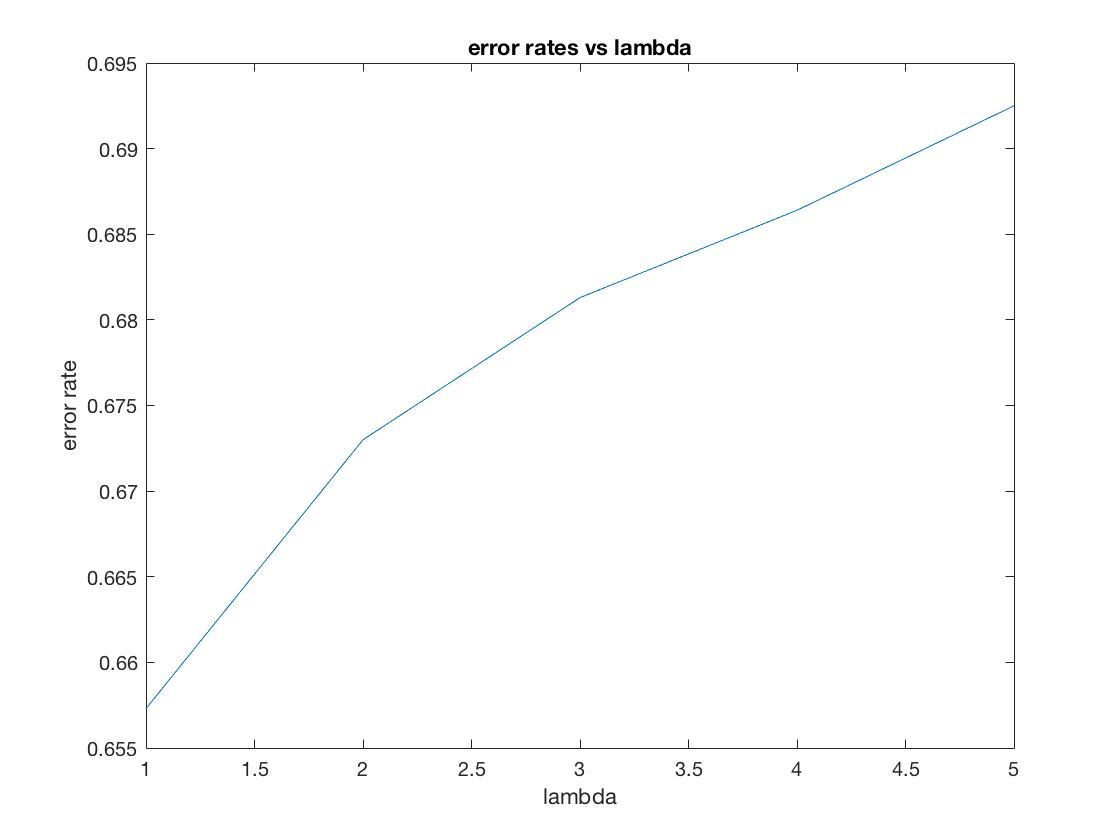
\includegraphics[scale = 0.4]{e12.jpg}

\subsection{Question 1.3}
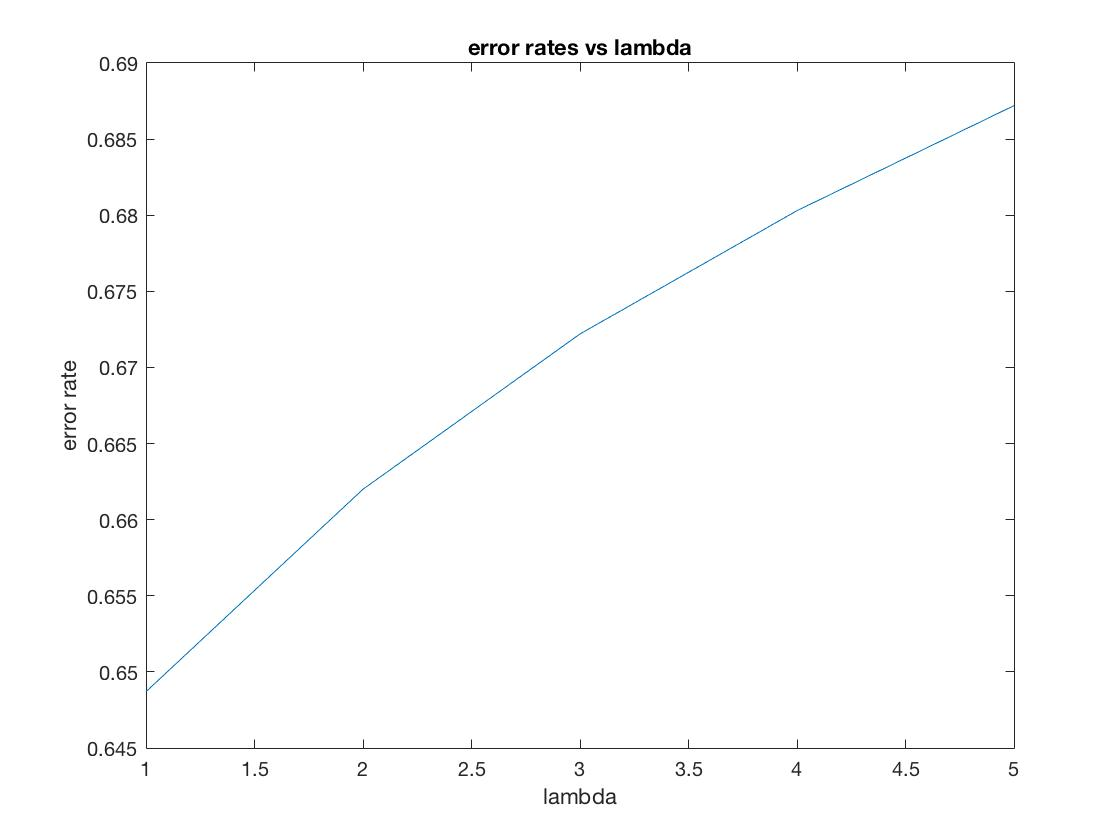
\includegraphics[scale = 0.4]{e13.jpg}

\subsection{Question 1.4}
For kernelized logistic regression, each $x$ is transformed to $\phi(x)$, and the weight is defined in terms of support vectors\\
\centerline{$w$ = $\sum_{i}\alpha_{i}\phi(x_{i})$}\\\\
Therefore, the sigmoid function is defined as \\\\
\centerline{$p$ = $\frac{1}{1+e^{-y_{i}\sum_{i}\alpha_{i}\phi(x_{i})\phi(x)}}$ = $\frac{1}{1+e^{-y_{i}\sum_{i}\alpha_{i}K(x,x_{i})}}$}\\\\
The the loss function of kernel logistic regression becomes:\\\\
\centerline{$\min_{w}\frac{1}{n^{+}}\sum_{i:y_{i}=1}log(1+exp(-y_{i}\sum_{l}\alpha_{l}K(x,x_{i})))+\frac{1}{n^{-}}\sum_{j:y_{j}=-1}log(1+exp(-y_{j}\sum_{l}\alpha_{l}K(x,x_{j})))$+$\lambda w^{t}w$}\\\\
To calculate the Gradient, we do the following:\\\\
\centerline{$\nabla f(\alpha)$ =$\frac{1}{n^{+}}\sum_{i:y_{i}=1}-p(x_{i})(\frac{1}{p(x_{i})}-1)y_{i}K(x,x_{i})$+$\frac{1}{n^{-}}\sum_{i:y_{j}=-1}-p(x_{j})(\frac{1}{p(x_{j})}-1)y_{j}K(x,x_{j})$+$2\lambda K\alpha $}\\\\
To calculate the Hessian, we do the following:\\\\
\centerline{let $s_{ks}$ = $\frac{\partial}{\partial \alpha_{s}}g_{k}$ }\\\\
\centerline{Then $s_{ks}$=$\frac{1}{n^{+}}\sum_{i:y_{i}=1}\frac{e^{-y_{i}\sum_{l}\alpha_{l}k(x,x_{i})}K(x_{k},x_{i})K(x_{s},x_{i})}{(1+e^{-y_{i}\sum_{l}\alpha_{l}K(x,x_{i})})^{2}}$+$\frac{1}{n^{-}}\sum_{j:y_{j}=-1}\frac{e^{-y_{i}\sum_{l}\alpha_{l}k(x,x_{j})}K(x_{k},x_{j})K(x_{s},x_{j})}{(1+e^{-y_{j}\sum_{l}\alpha_{l}K(x,x_{j})})^{2}}$+$2\lambda K(x_{k},x_{s})$}\\\\
\centerline{Therefore}\\\\
\centerline{$s_{ks}$ =$\frac{1}{n^{+}}\sum_{i:y_{i}=1}(p(x_{i})-p^{2}(x_{i}))K(x_{k},x_{i})K(x_{s},x_{i})$+$\frac{1}{n^{-}}\sum_{j:y_{j}=-1}(p(x_{j})-p^{2}(x_{j}))K(x_{k},x_{j})K(x_{s},x_{j})$+$2\lambda K(x_{k},x_{s})$}\\\\
\centerline{$\nabla^{2} f(\alpha)$ = \[
$\begin{bmatrix}
    s_{11} & s_{12}&...&s_{1d}\\
    s_{21} & s_{22}&...&s_{2d}\\
   ... \\
    s_{d1} & s_{d2}&...&s_{dd}\\
\end{bmatrix}
$\]}\\\\

For linear kernel, we have:\\\\
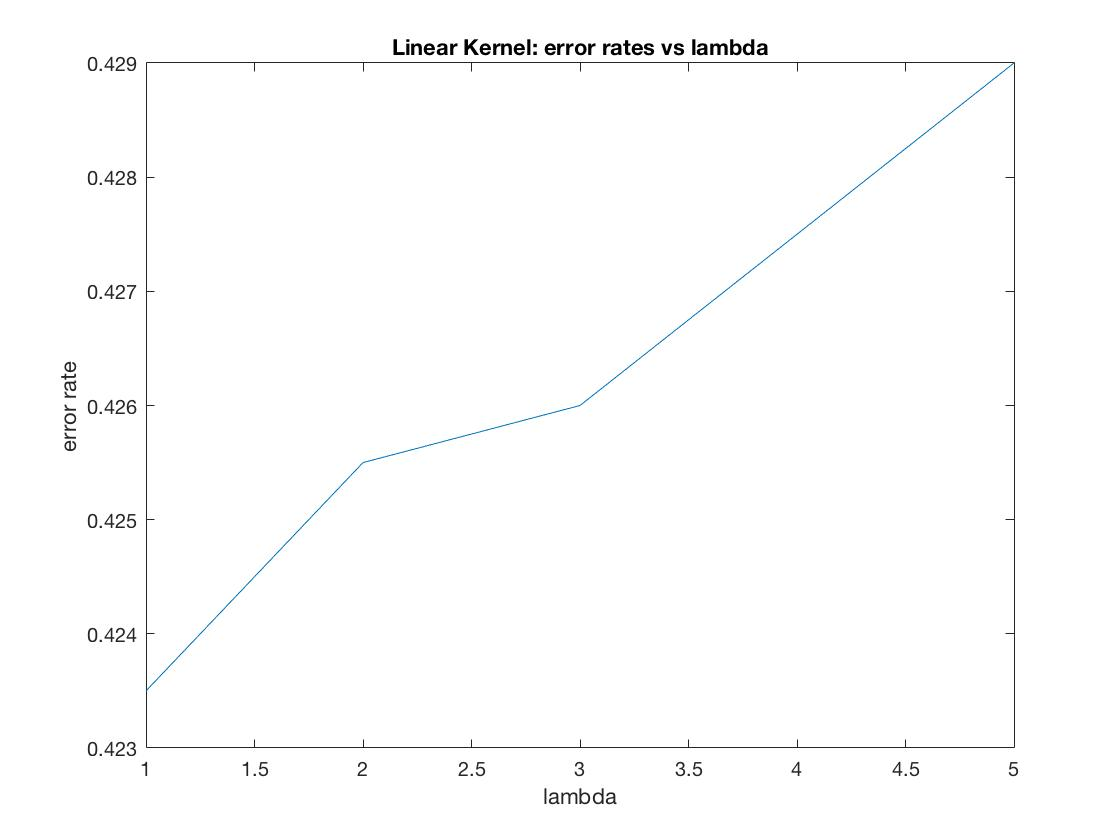
\includegraphics[scale = 0.4]{e14linear.jpg}
For polynomial kernel, we have(The error rate maintains $42.35\%$ for all $\lambda$ values from 1 to 5):\\\\
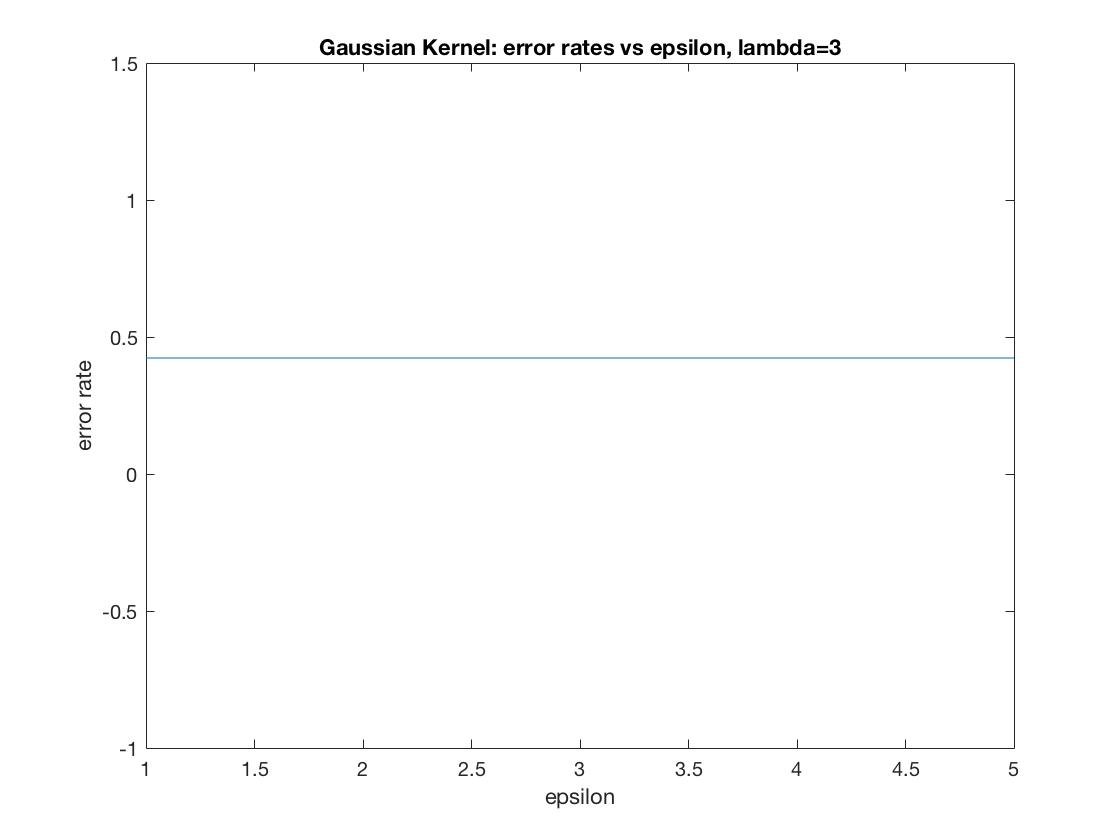
\includegraphics[scale = 0.4]{e14polynomial.jpg}
For Gaussian kernel, when $\lambda = 1$, we have:\\\\
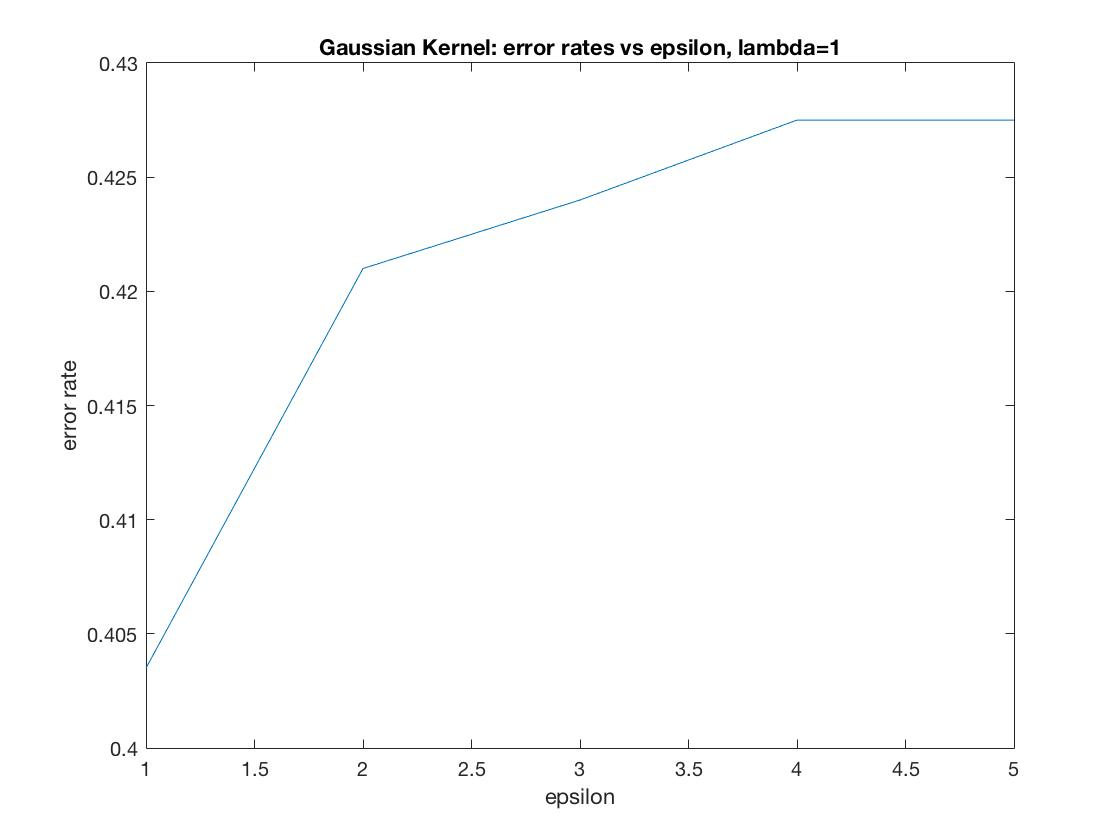
\includegraphics[scale = 0.4]{e14gaussianlambda1.jpg}
For Gaussian kernel, when $\lambda = 3$, we have:\\\\
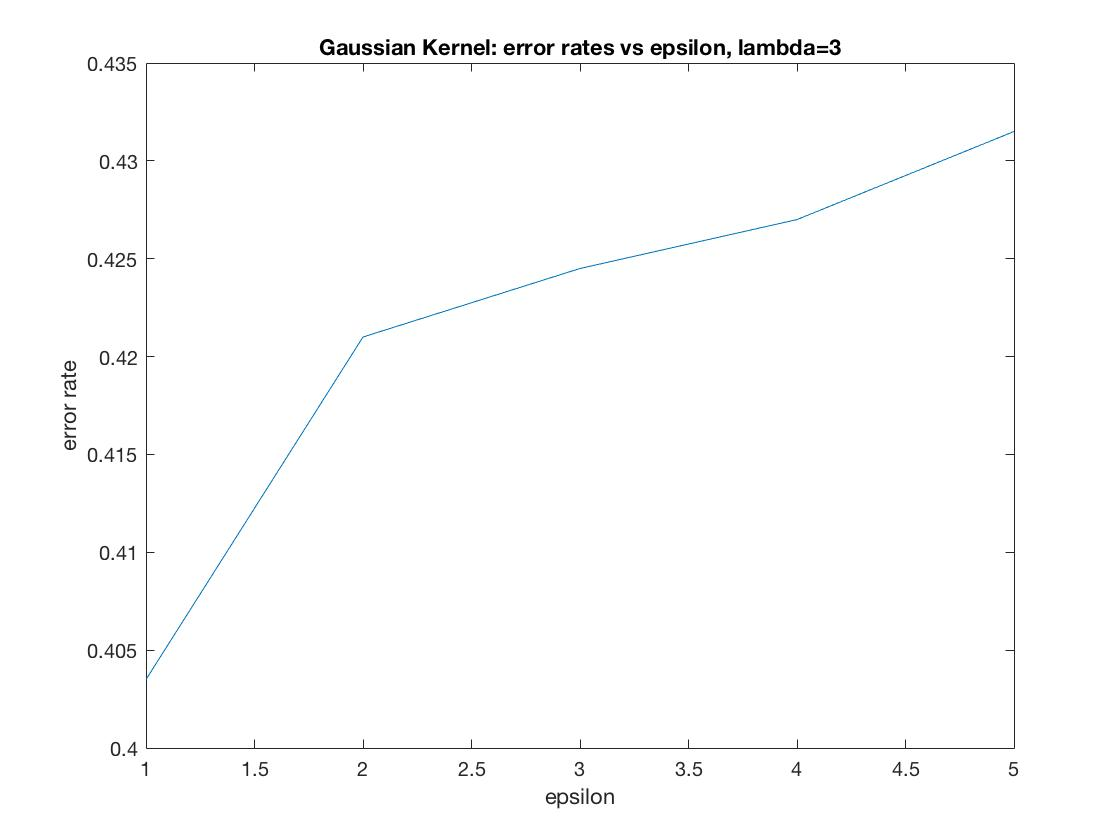
\includegraphics[scale = 0.4]{e14gaussianlambda3.jpg}
For Gaussian kernel, when $\lambda = 5$, we have:\\\\
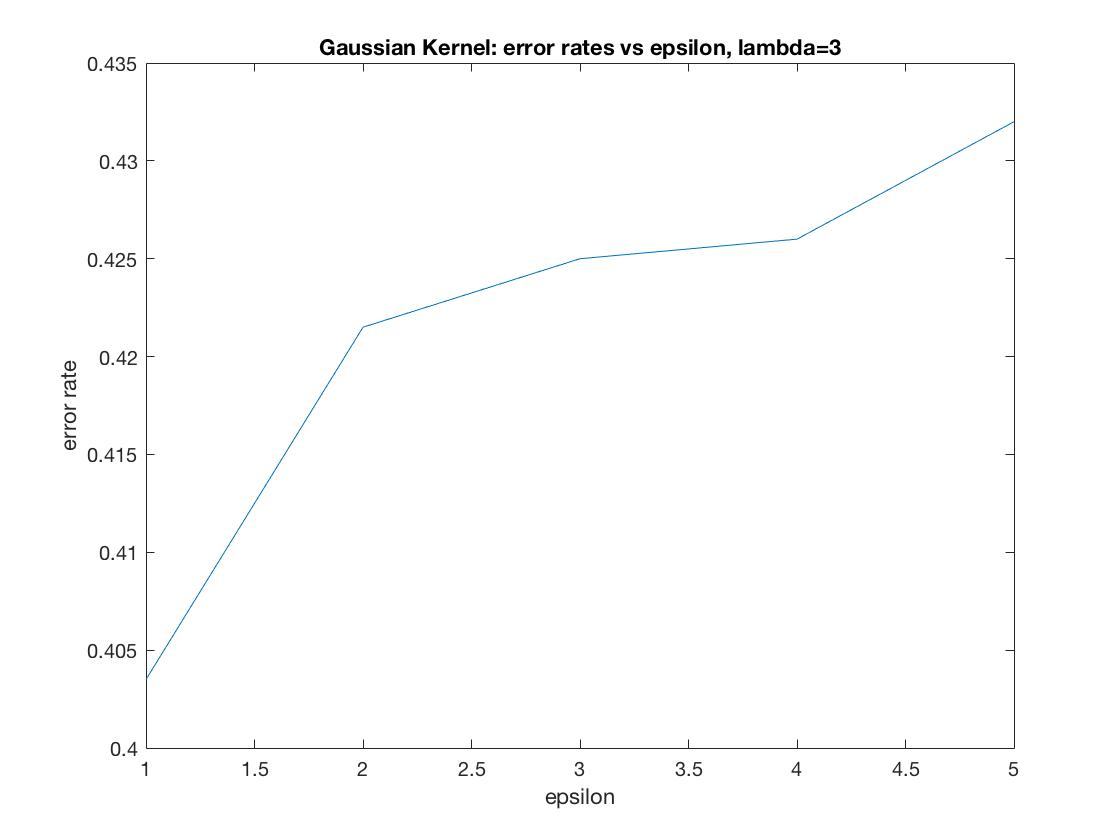
\includegraphics[scale = 0.4]{e14gaussianlambda5.jpg}

\section{Exercise 2}
\subsection{Question 2.1}
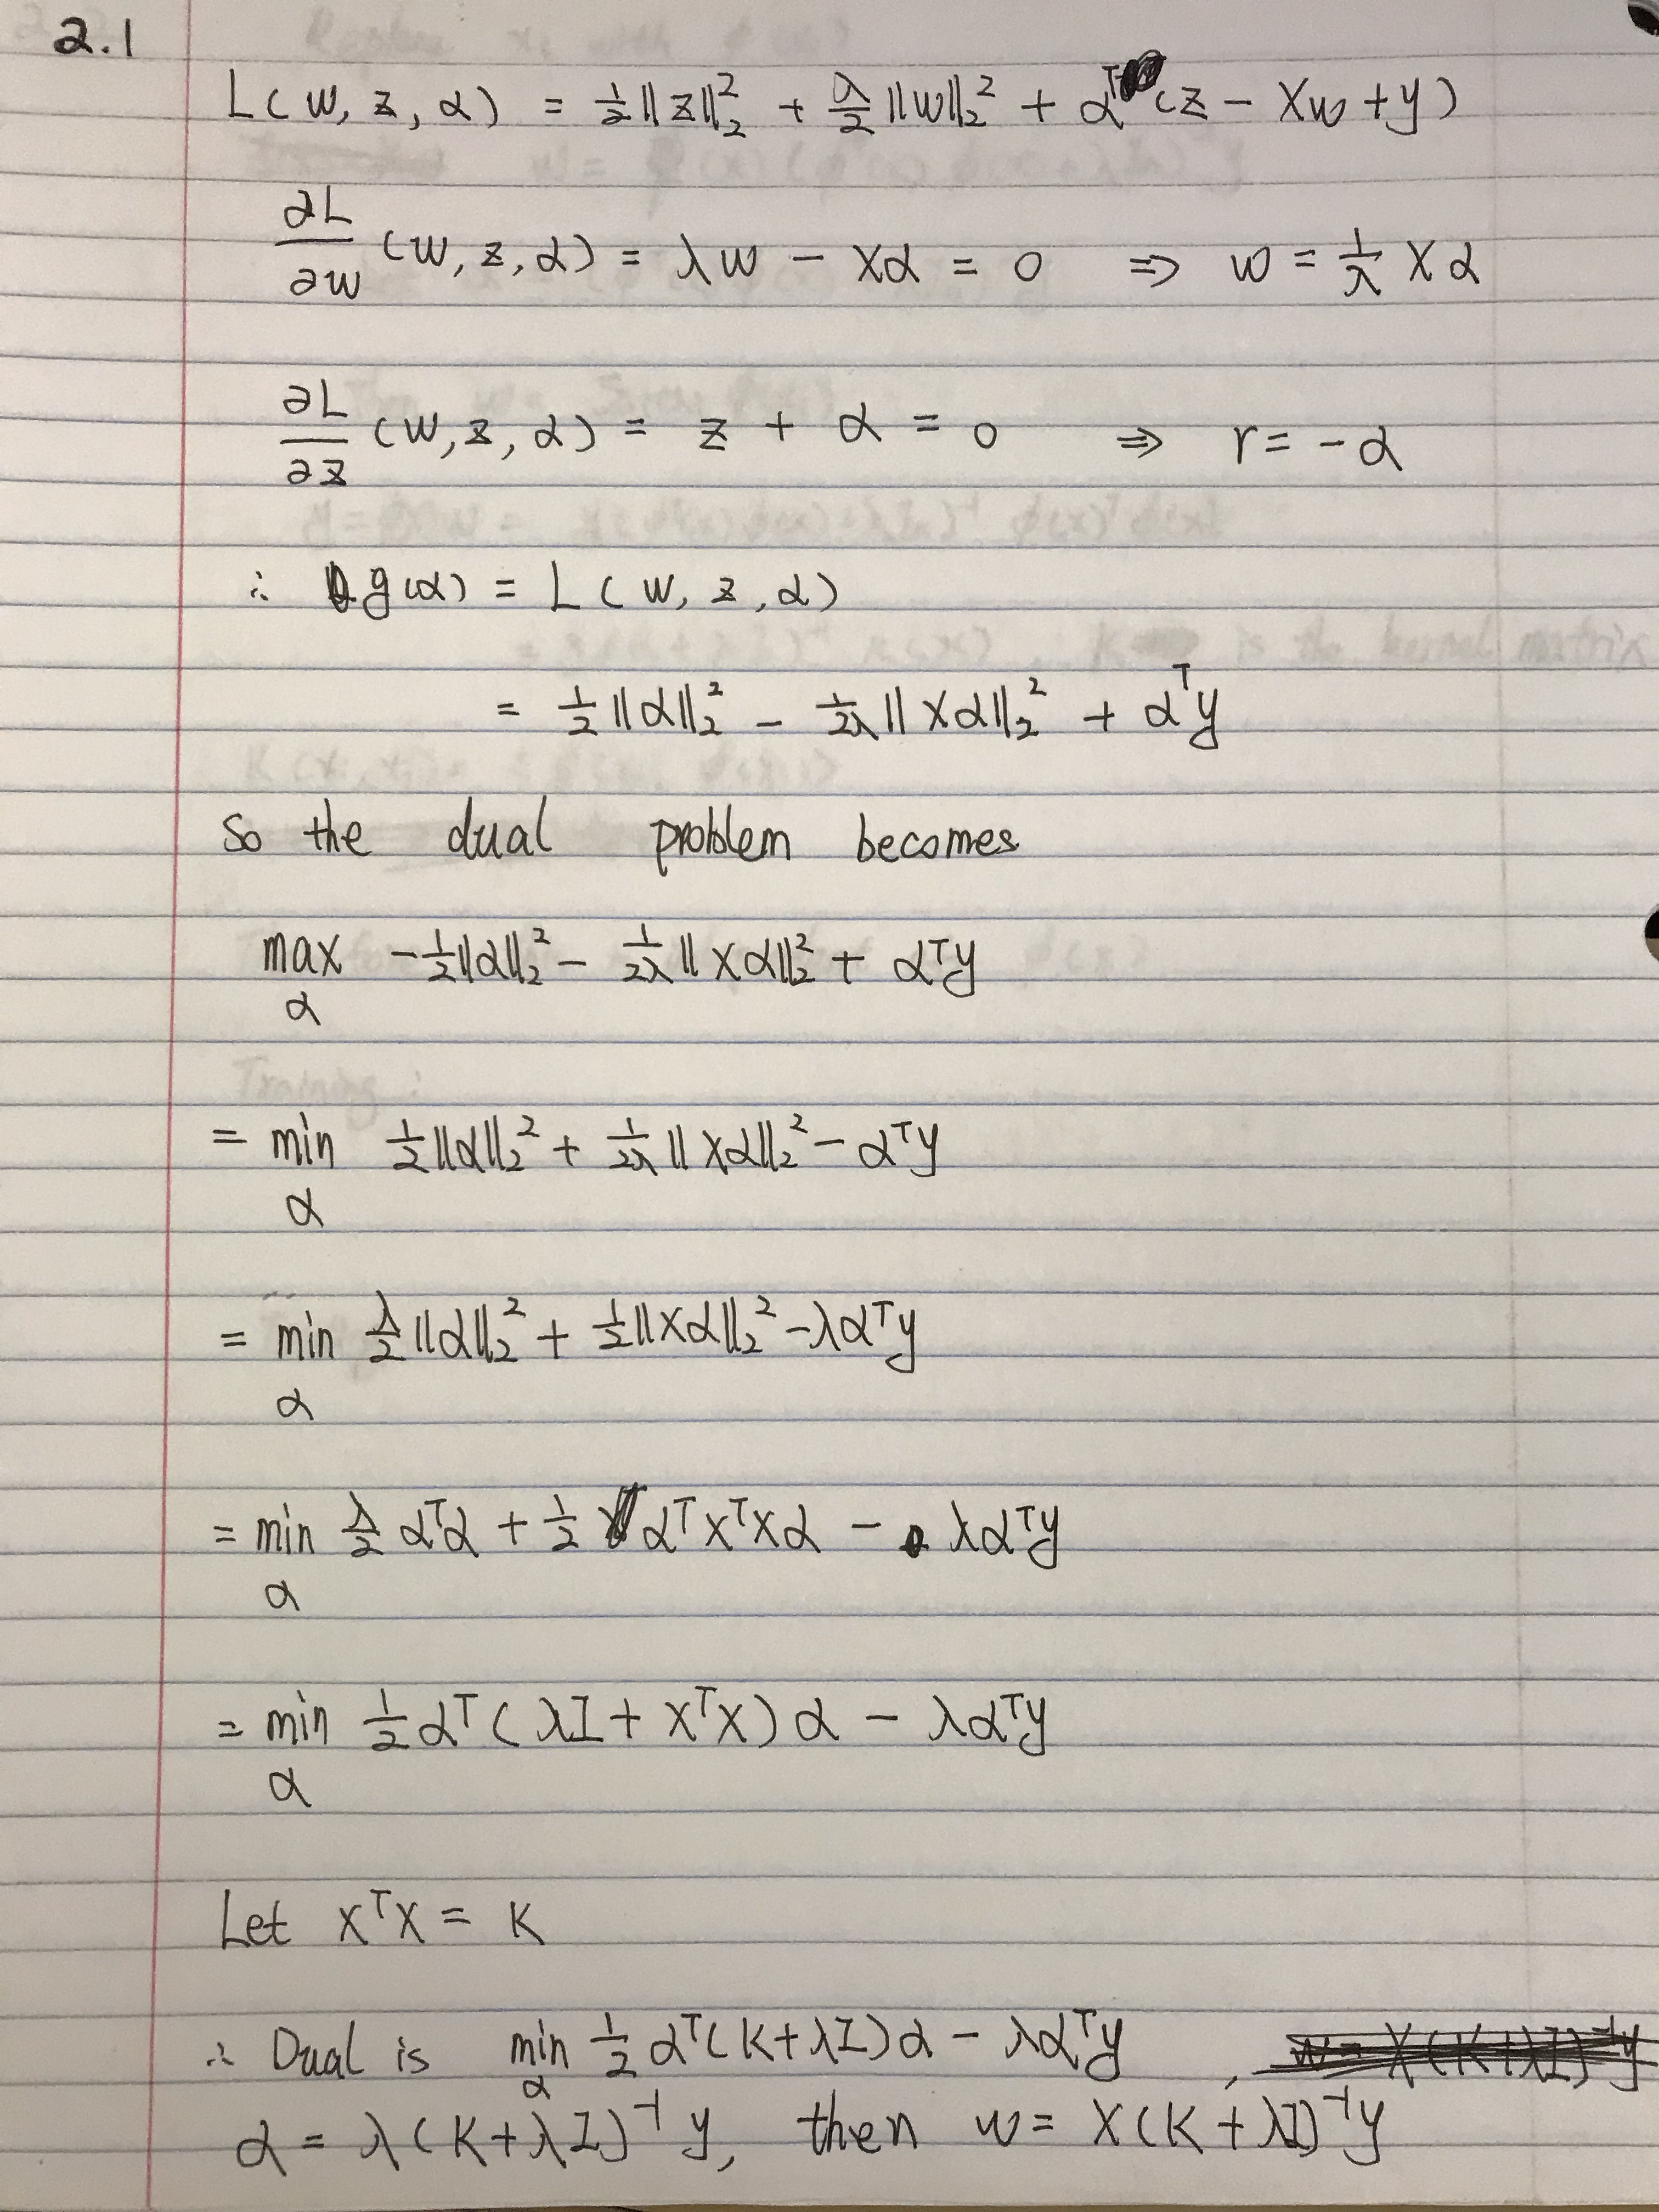
\includegraphics[scale = 0.15]{e21.jpeg}

\subsection{Question 2.2}
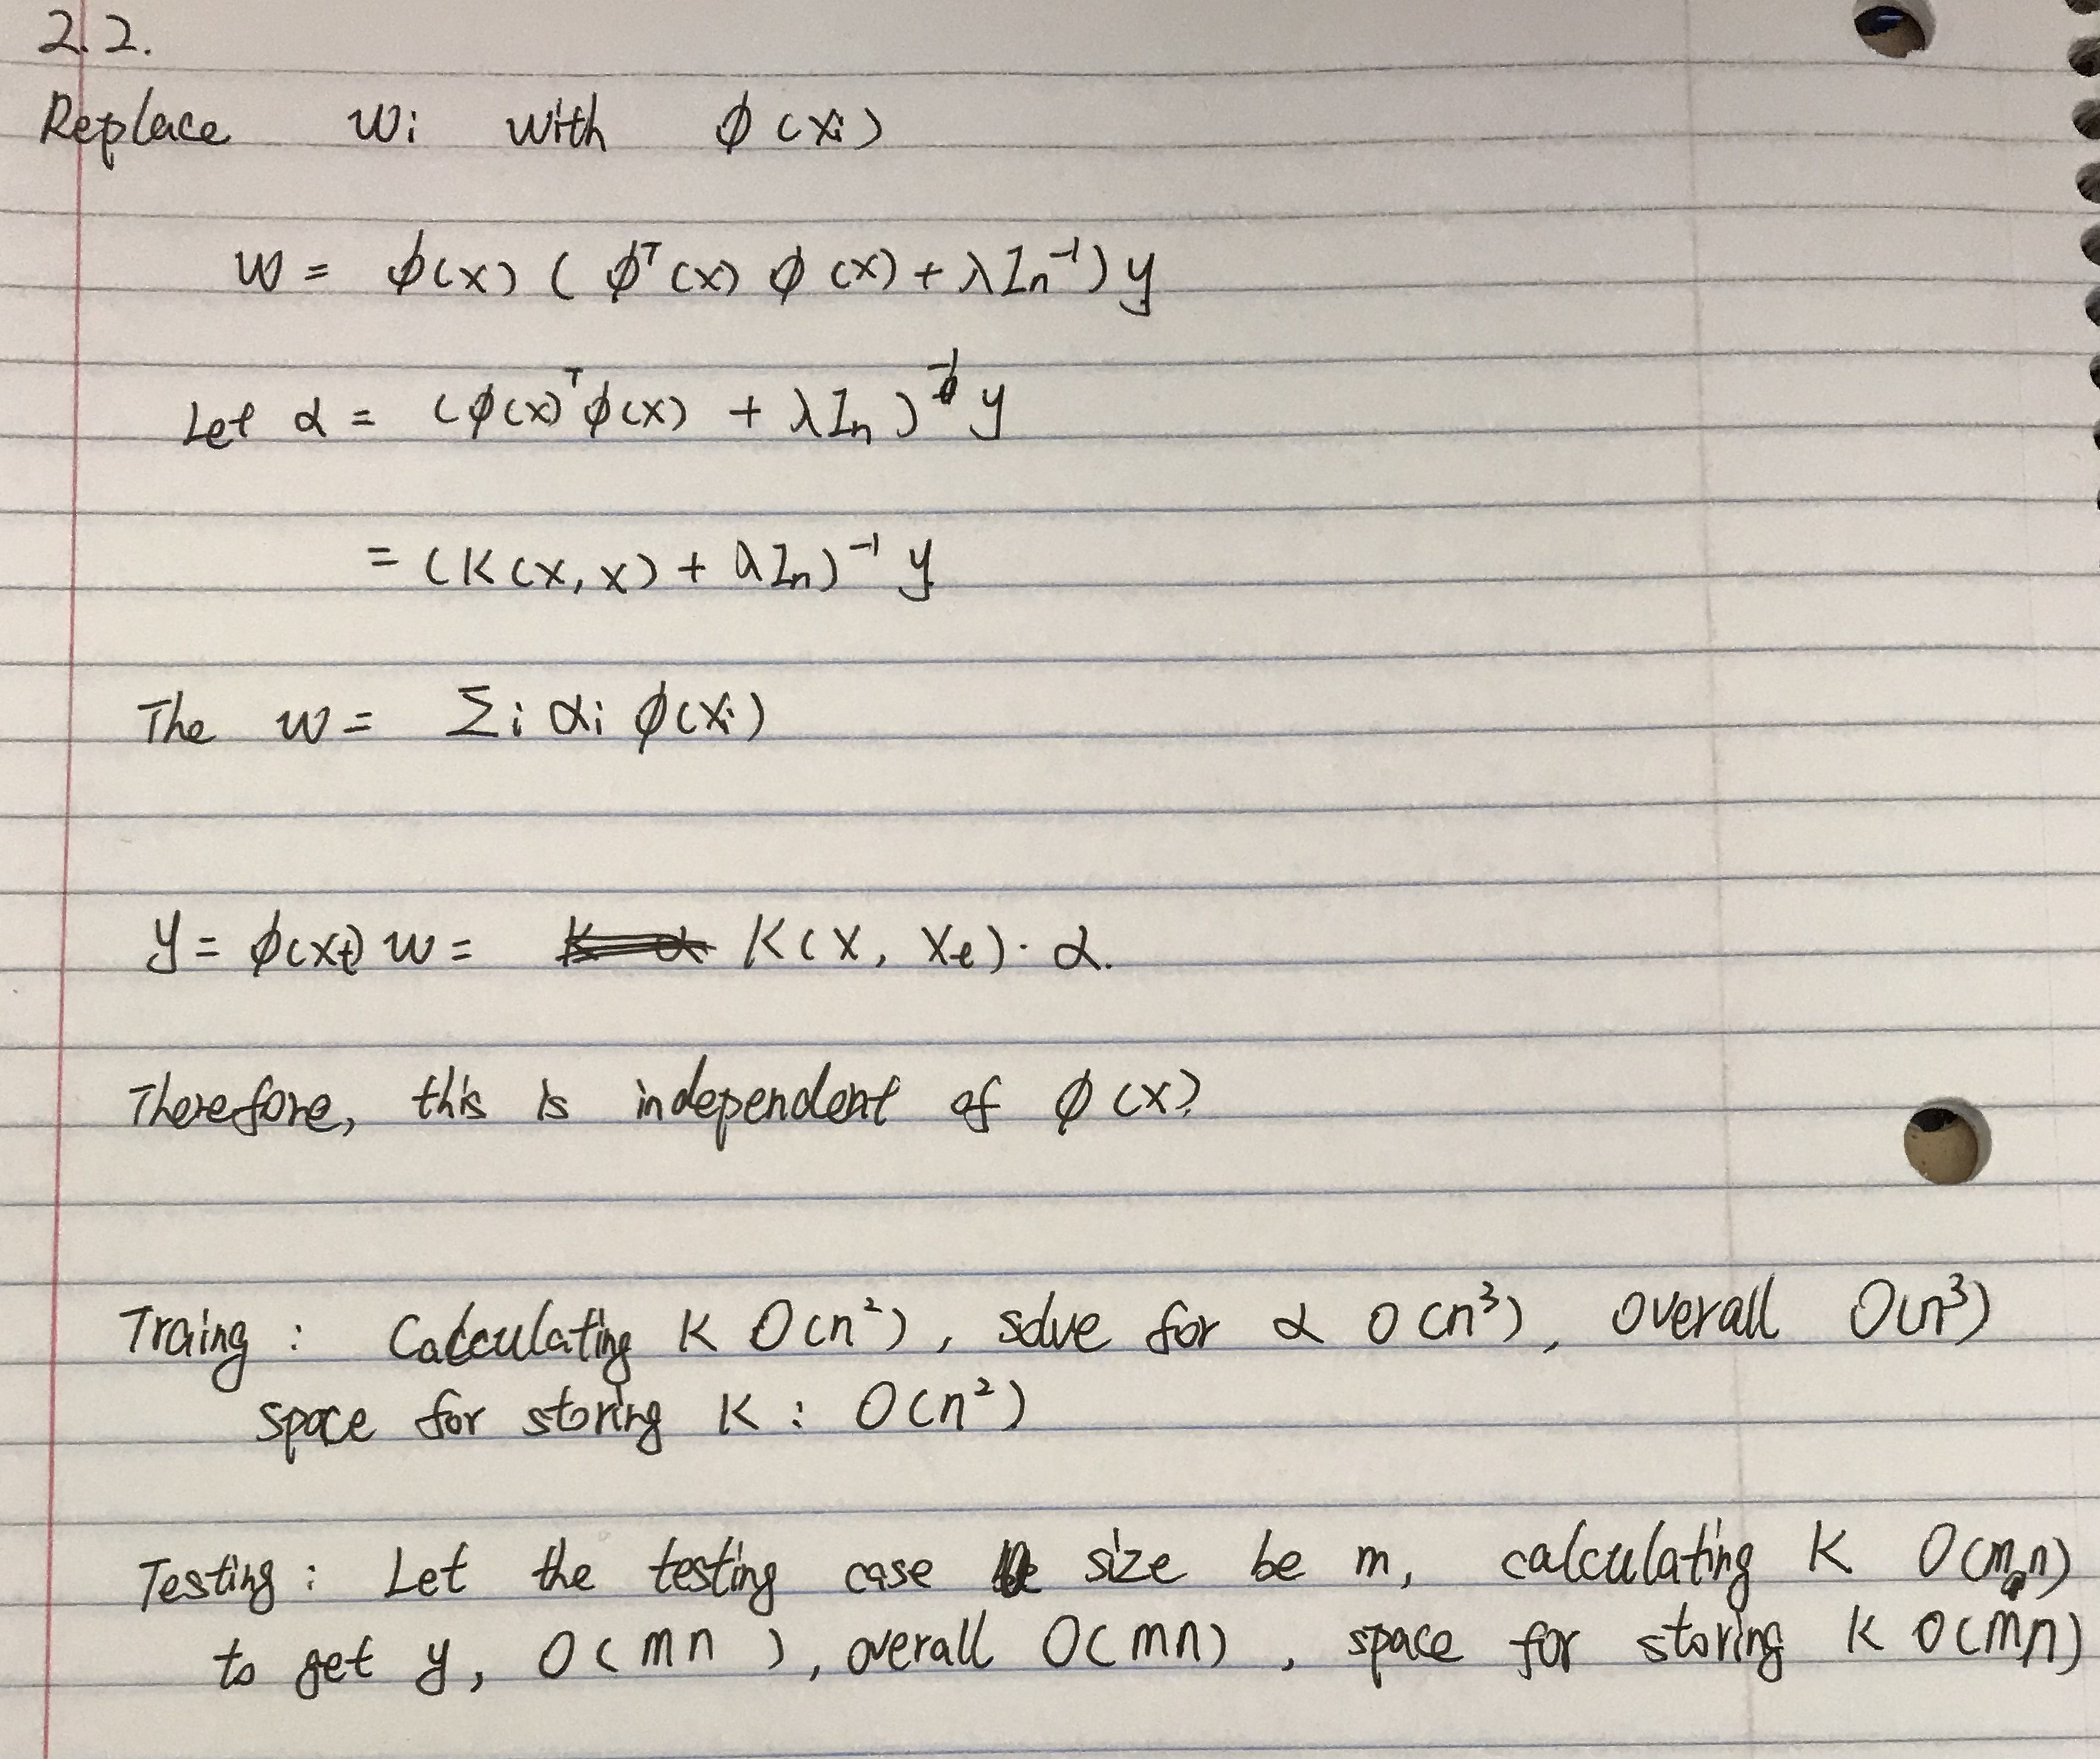
\includegraphics[scale = 0.15]{e22.jpeg}

\subsection{Question 2.3}
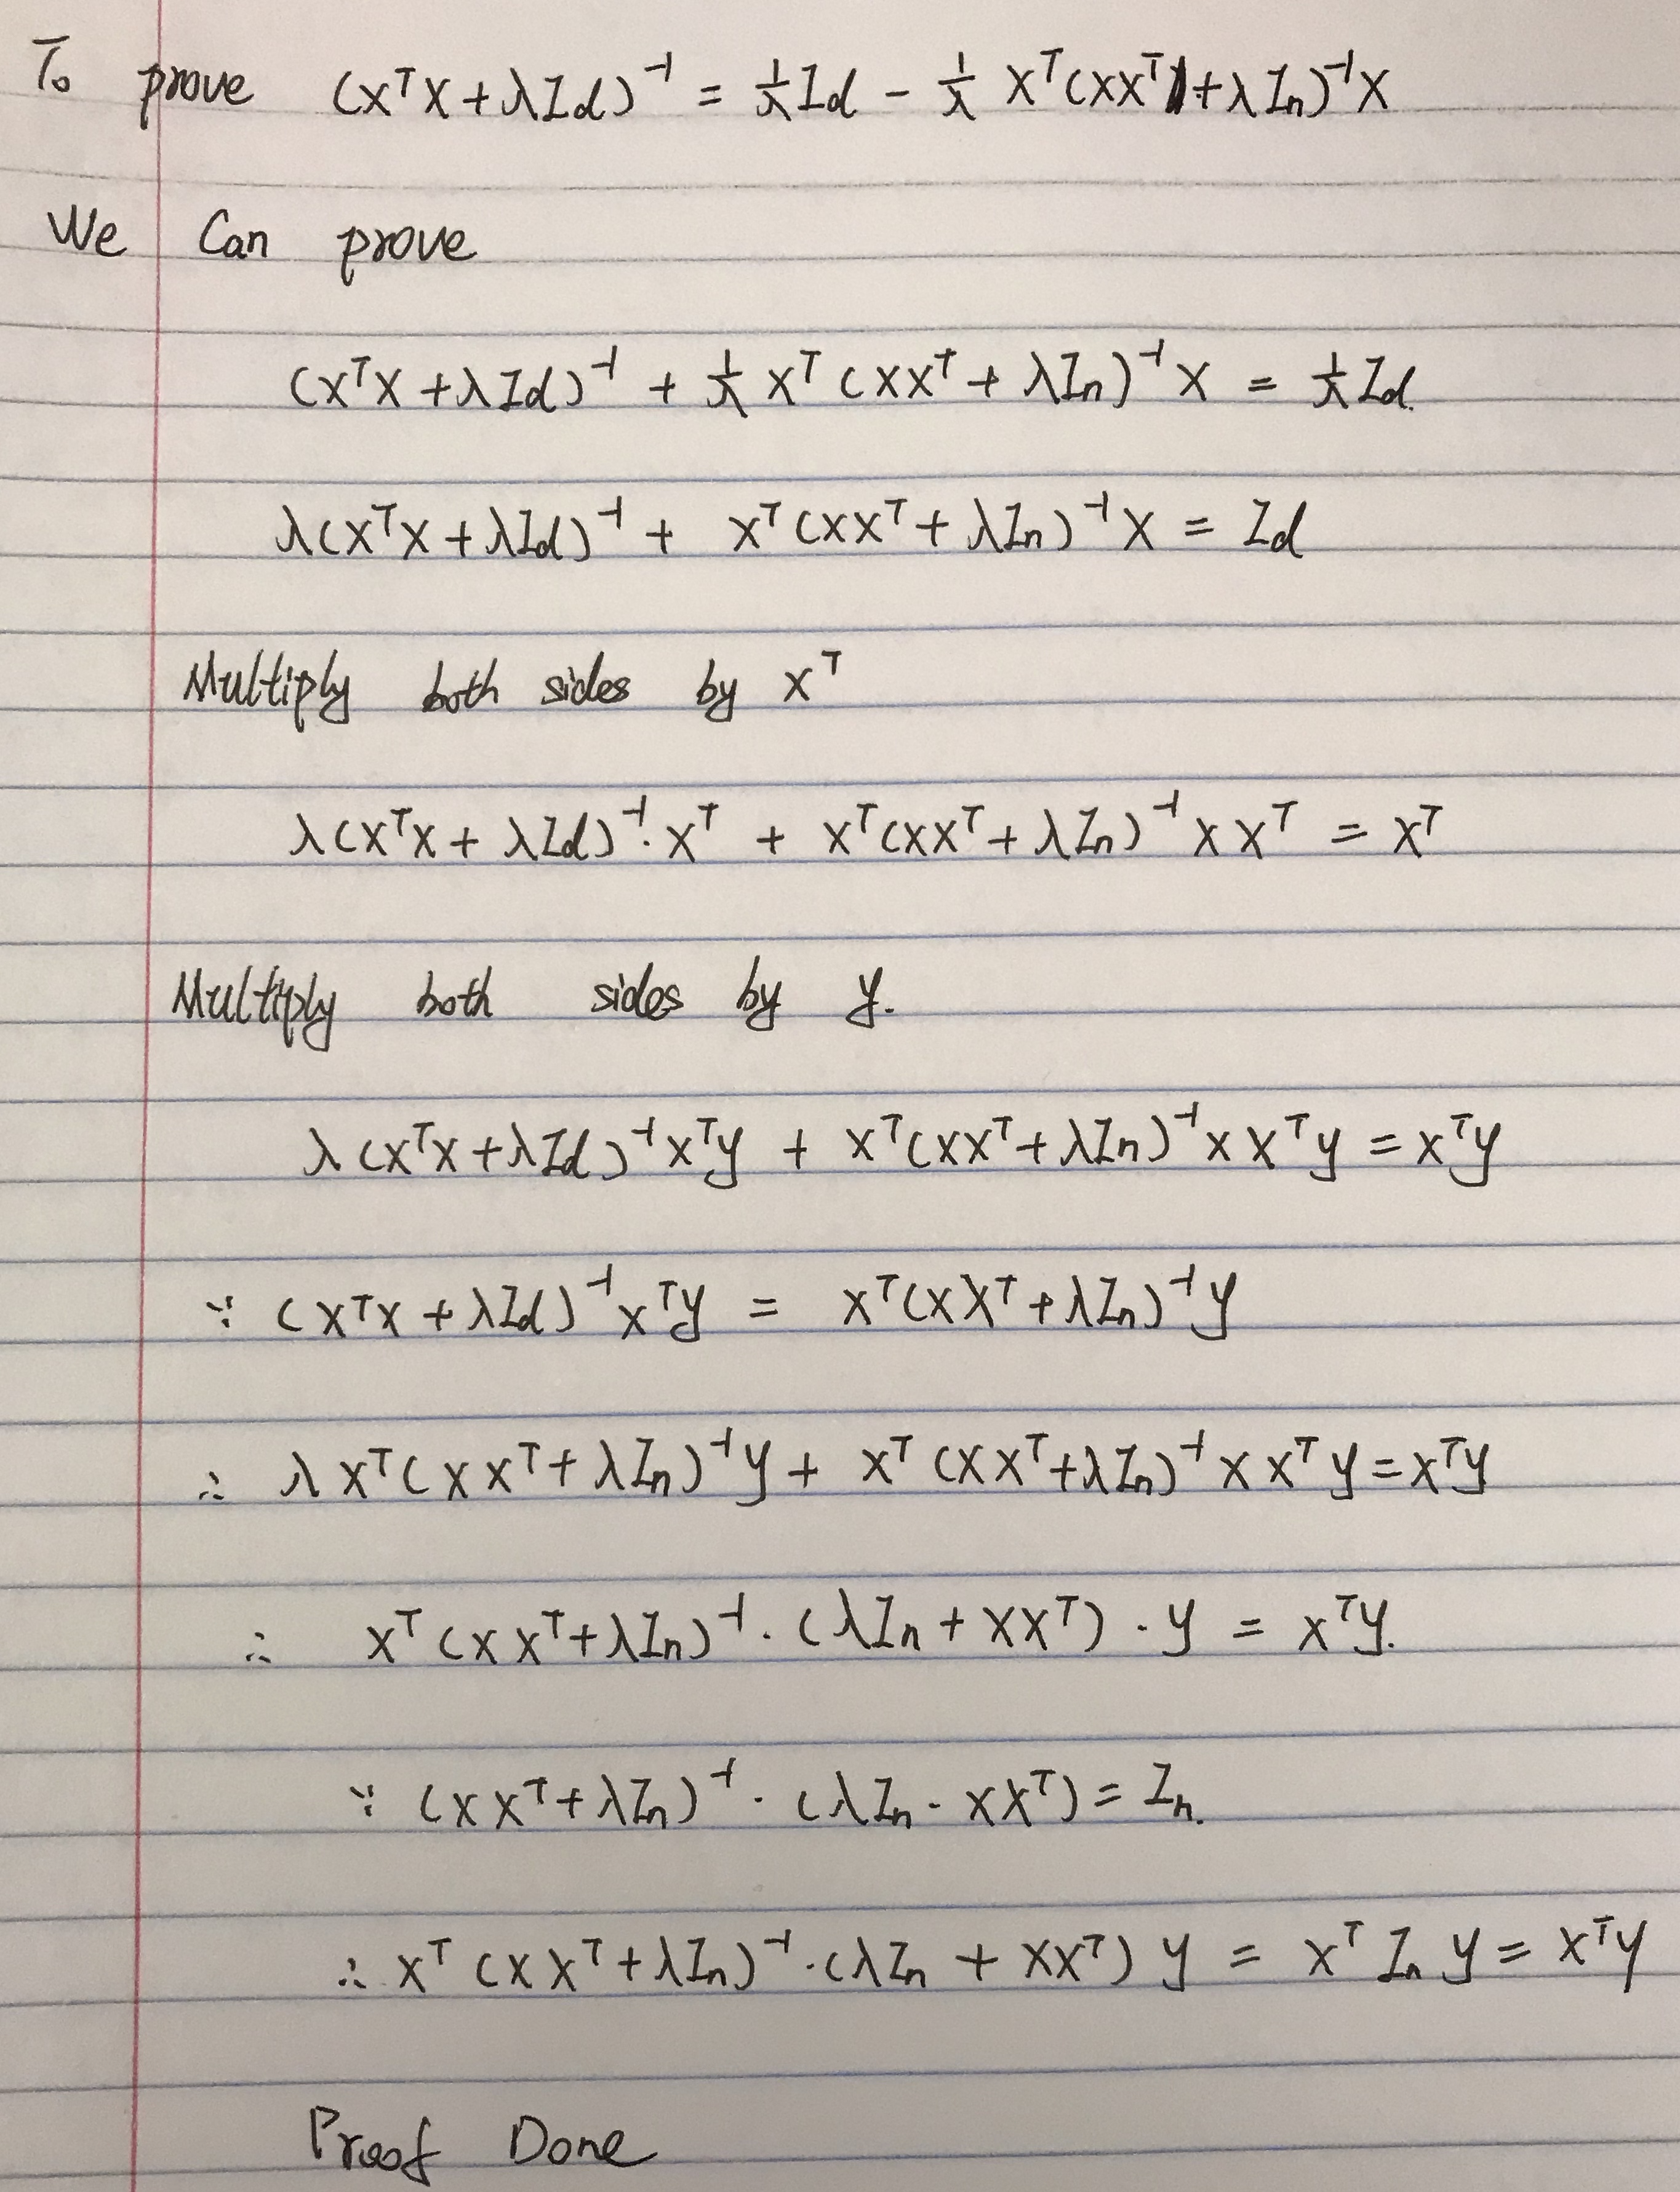
\includegraphics[scale = 0.15]{e23.jpeg}

\section{Exercise 3}
\subsection{Question 3.1}
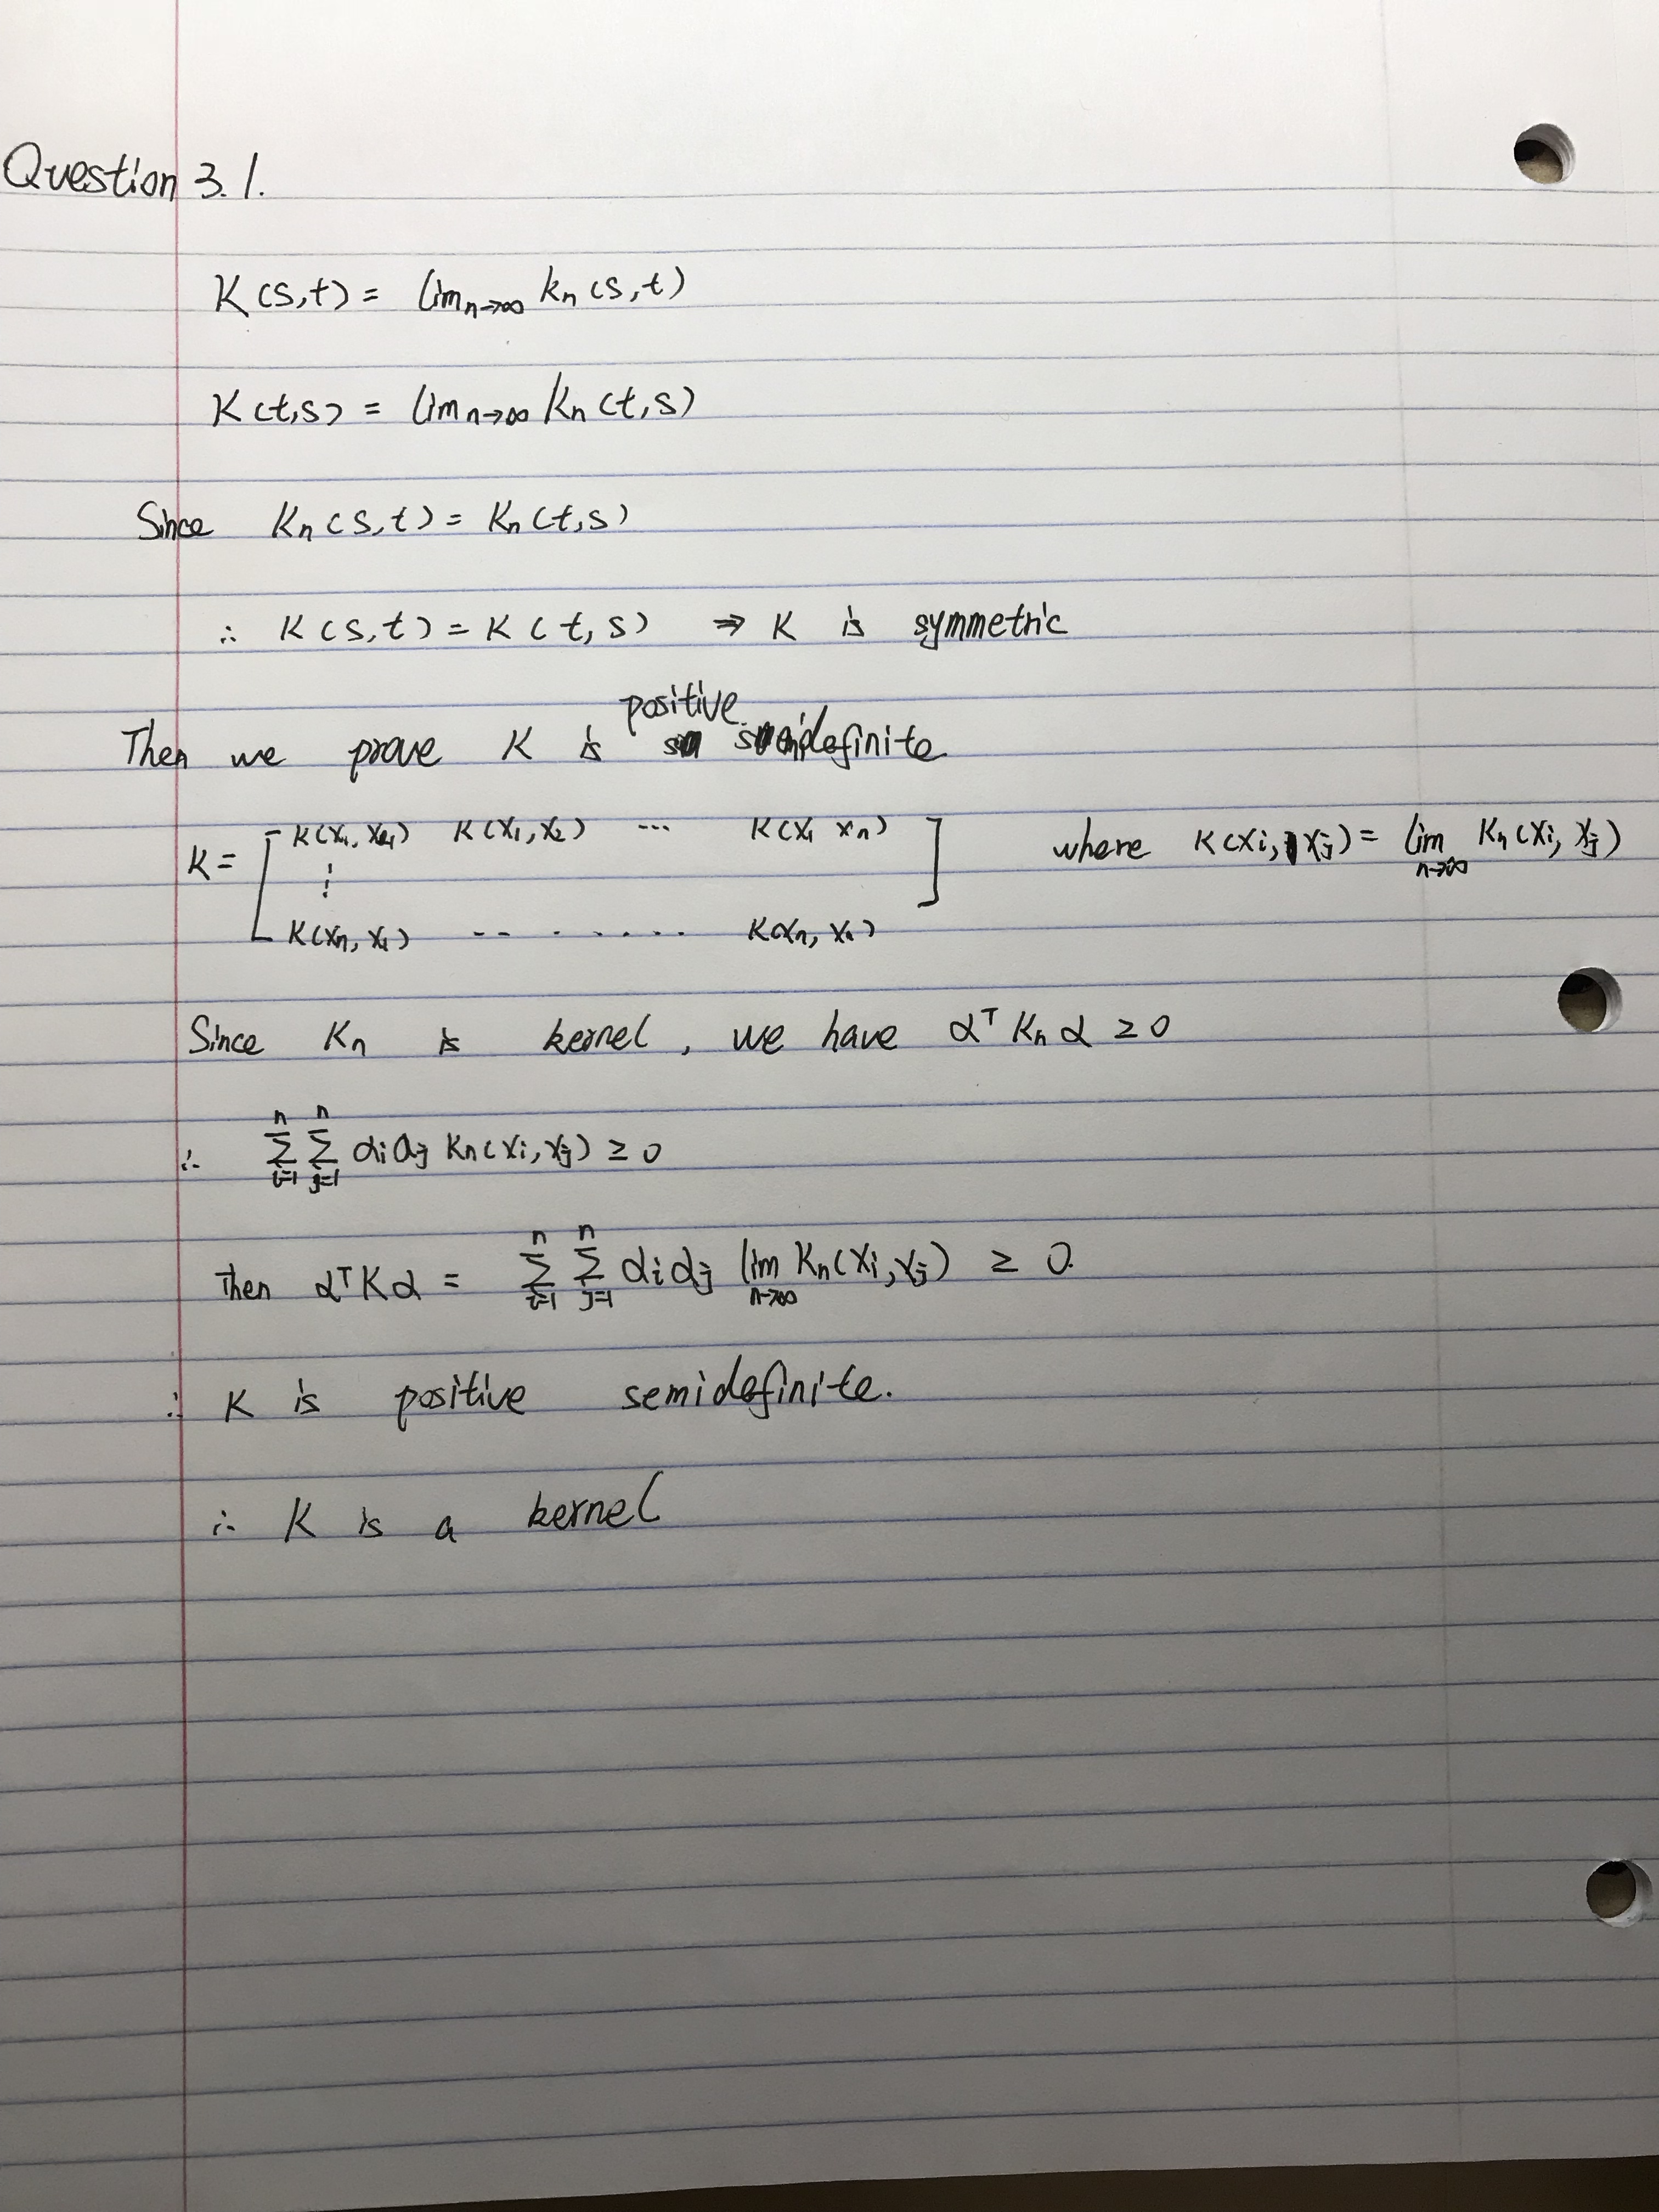
\includegraphics[scale = 0.15]{e31.jpeg}

\subsection{Question 3.2 \& 3.3}
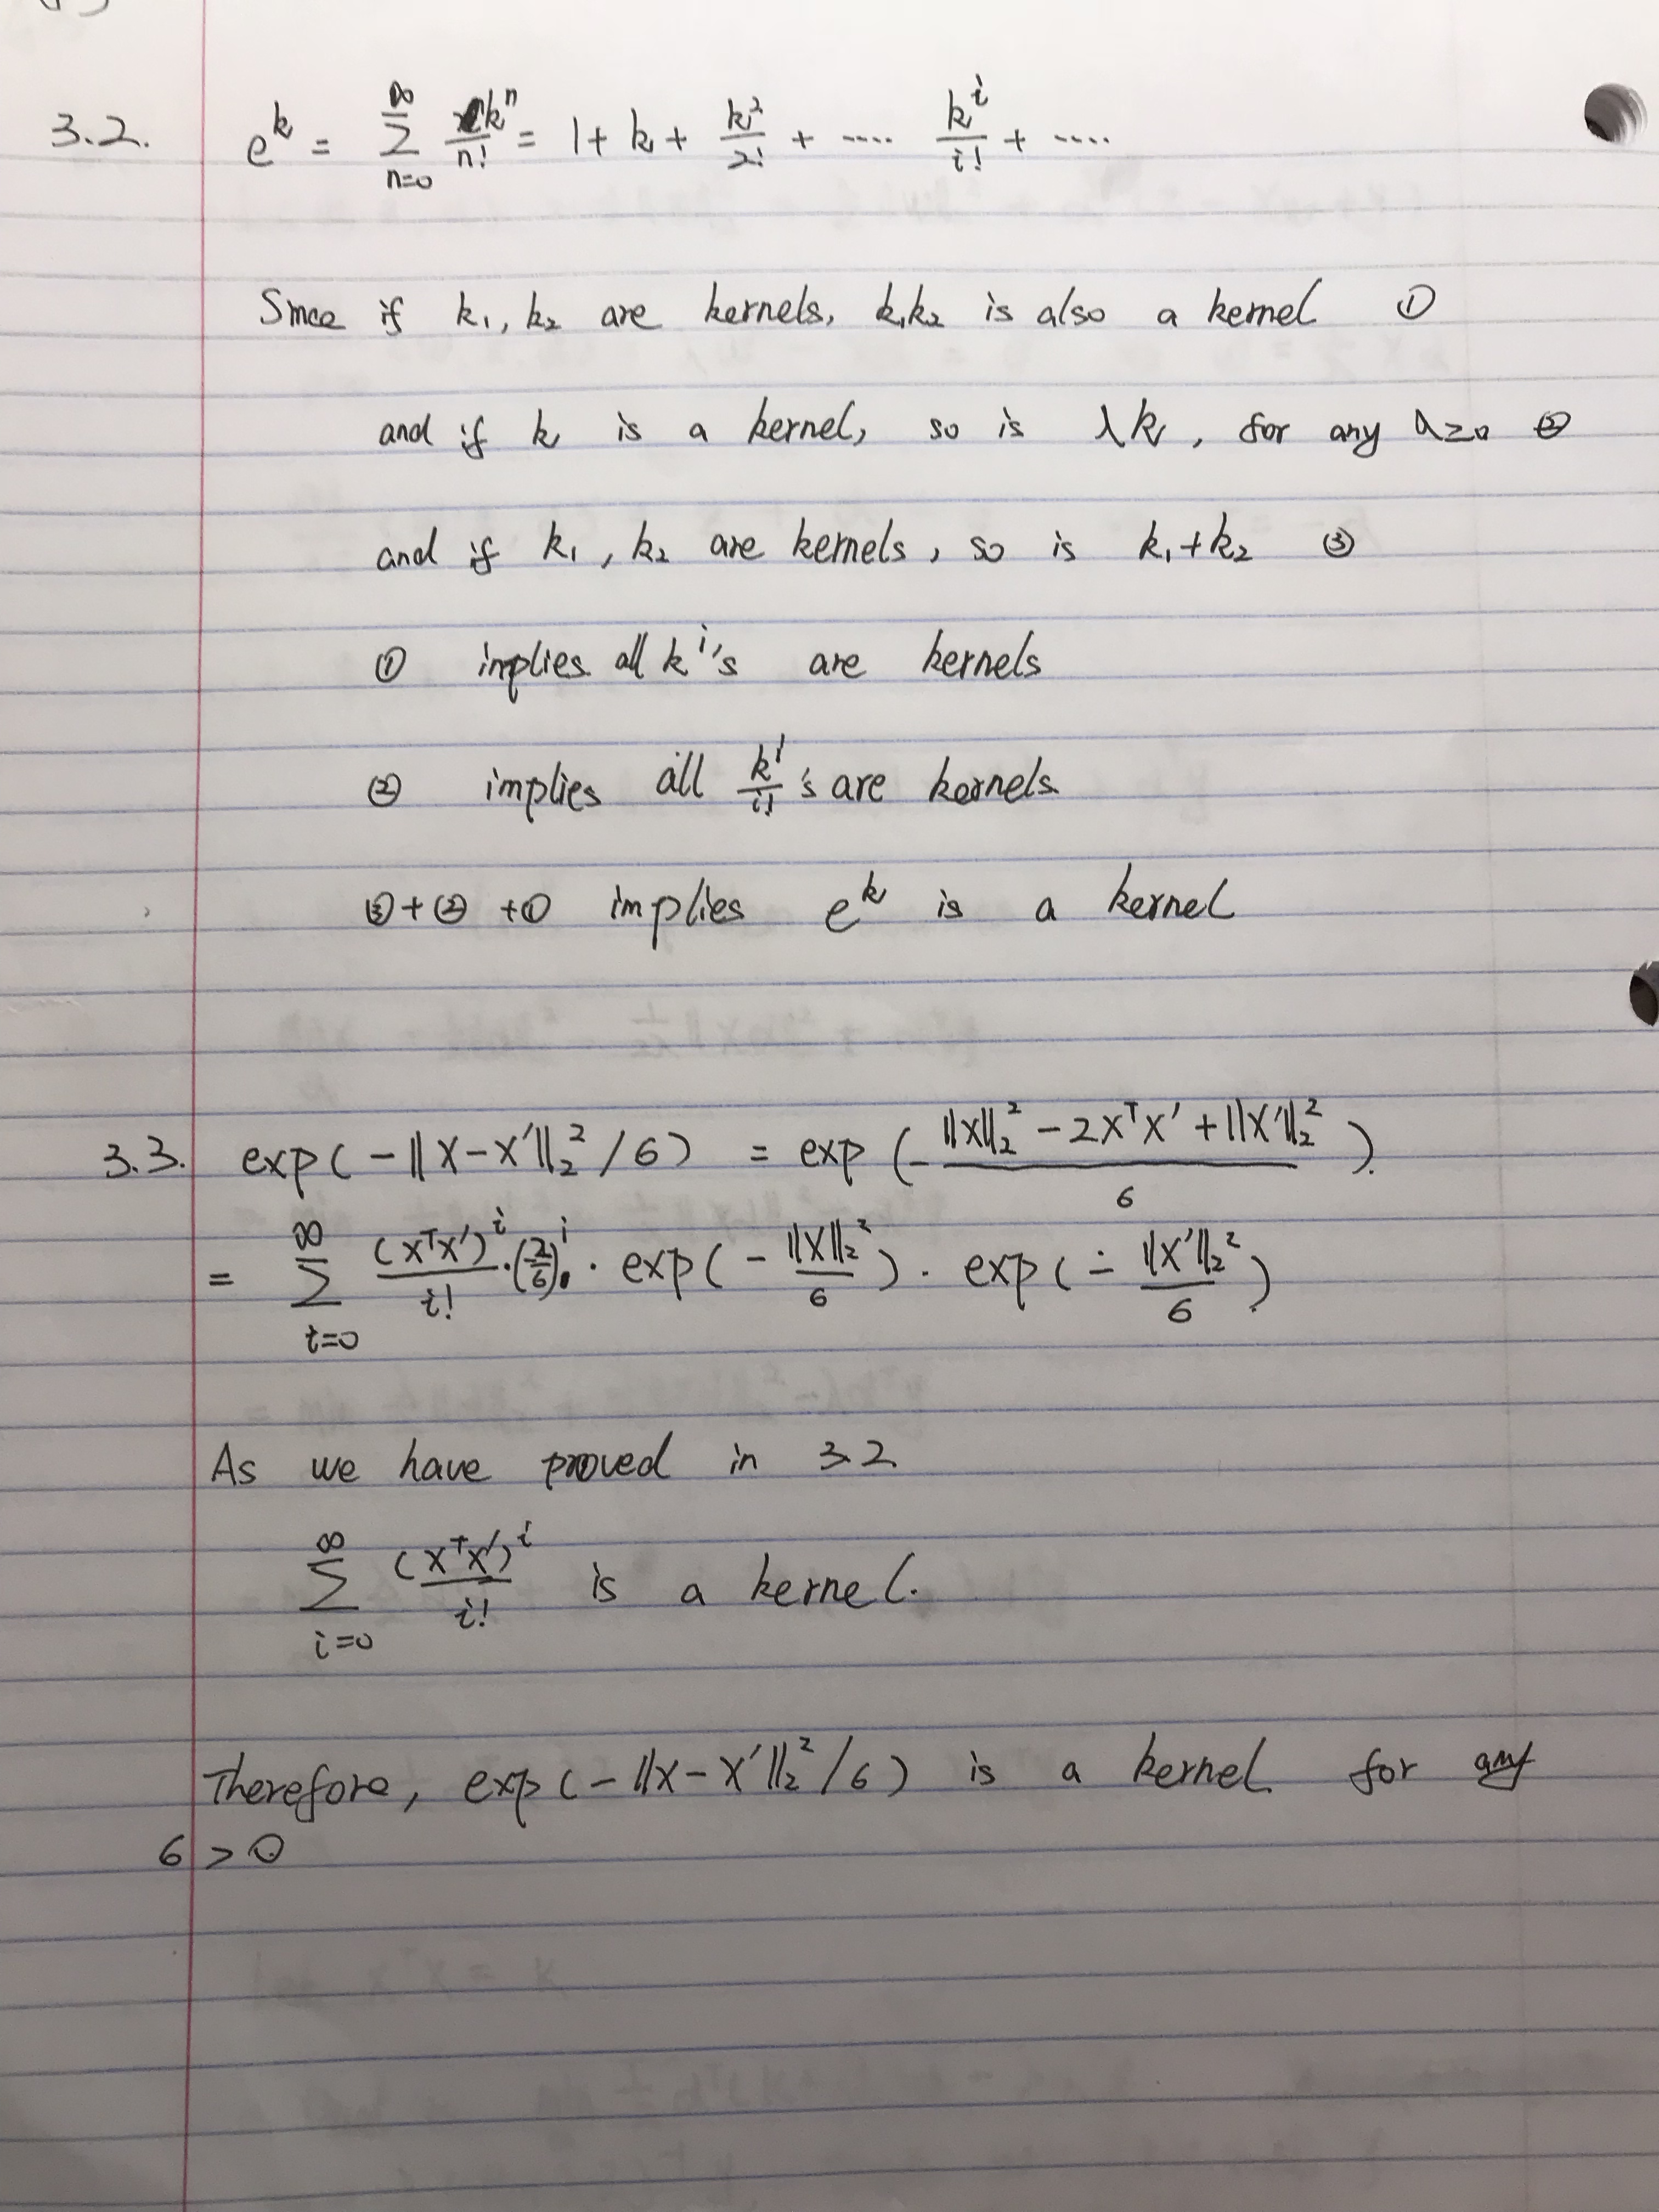
\includegraphics[scale = 0.15]{e32.jpeg}


\end{document}
